% !TeX root = bachelorarbeit.tex
 \label{DG}
In diesem Abchnitt soll nun, nachdem wir $q(\omega,\cdot)$ als Finite-Elemente-Lösung des Potentialströmungsproblems erhalten haben, die numerische Lösung des linearen Transportproblems behandelt werden:
\begin{align*}
	&\text{Für } \omega \in \Omega \text{ und }q(\omega,\cdot): \overline{\mathcal{D}} \to \R^2 \text{, bestimme }\rho(\omega,\cdot): \overline{\mathcal{D}} \times \mathbb{T} \to \R_{\geq 0} \text{ mit} \\
	&\text{(pTP)} 
	\begin{cases}
	\begin{array}{rlll}
	\partial_t \rho (\omega, x, t) + \dive(\rho(\omega,x,t)q(\omega,x)) &= 0 &\text{, für } (x,t) \in \mathcal{D} \times (0,T] \\
	\rho(\omega,x,t) &= \rho_{\text{in}}(x,t) &\text{, für } (x,t) \in \Gamma_{\text{in}} \times \mathbb{T} \\
	\rho(\omega,x,0)  &= \rho_0(x) &\text{, für } x \in  \mathcal{D}
	\end{array}
	\end{cases} \\
\end{align*}
Insbesondere wollen wir an dieser Stelle wieder $\omega \in \Omega$ festhalten und betrachten deshalb zunächst nur das deterministische Problem wie in \ref{det_prob}:
\[ 
\text{Bestimme } \rho: \overline{\mathcal{D}} \times \mathbb{T} \to \R_{\geq 0} \text{, sodass} \newline \]
\[\setlength\arraycolsep{1pt}
\text{(dTP)}\begin{cases} 
\begin{array}{rlll}
\partial_t \rho(x,t) + \dive(\rho(x,t) q(x)) &= 0 &\text{ ,in } &\mathcal{D} \times (0,T)\\
\rho(x,t) &= \rho_{\text{in}}(x,t) &\text{ ,auf } &\Gamma_{\text{in}} \times (0,T)\\
\rho(x,0) &= \rho_0(x) &\text{ ,auf } &\mathcal{D} \\
\end{array}
\end{cases} \\
\]
 Wir greifen dabei auf ein sogenanntes discontinuous Galerkin Verfahren zurück, welches für diese Problemklasse bereits an anderen Stellen (z.B. in \cite{cockburn1998runge}) erprobt wurde. Ursprünglich geht das Discontinuous Galerkin Verfahren auf Reed und Hill \cite{reed1973triangular} zurück. Einen guten (wenn auch mittlerweile etwas in die Jahre gekommenen) Überblick über die Anwendung von discontinuous Galerkin Verfahren bietet \cite{cockburn2000development}.
Grundätzlich handelt es sich beim discontinuous Galerkin Verfahren ebenfalls um einen FEM Ansatz, der zwar Ähnlichkeiten zum Finite Elemente Verfahren aufweist, welches wir im letzten Abschnitt gesehen hatten, aber auch einige bedeutende Unterschiede besitzt, auf welche wir im Folgenden besonders eingehen wollen. 
%So werden wir wieder eine schwache Formulierung des analytischen Problems herleiten und uns dann im Rahmen des diskretisierung erneut auf endlich dimensionale Räume zurückziehen.
Anders als zuvor das Potentialströmungsproblem ist die lineare Transportgleichung  nämlich sowohl orts- als auch zeitabhängig. Daher werden wir
%, nachdem wieder zuerst eine schwache Formulierung eingeführt wird,
  die lineare Transportgleichung zunächst im Ort diskretisieren. Wir erhalten so eine Semidiskretisierung, welche wir anschließend mit einem Zeitintegrator, wie beispielsweise der impliziten Mittelpunktsregel, in eine Volldiskretisierung überführen.
 

%\subsubsection{Schwache Formulierung}
%Wie im letzten Abschnitt führen wir nun einen schwachen Lösungsbegriff ein. Sei dazu $ \phi : \mathcal{D} \times \mathbb{T} \to \R $ eine beliebige Testfunktion, etwa aus  $W_0^{1,2}(\mathcal{D} \times \mathbb{T}) $, für die $ \phi(\cdot,T) = 0 $ gelte. 
%Wir beginnen mit der differentialgleichung $ \partial_t \rho(x,t) + \dive(\rho(x,t) q(x)) = 0  $, multiplizieren zunächst mit der Testfunktion $ \phi $ und integrieren anschließend über den Raum-Zeitzylinder $ \mathcal{D} \times \mathbb{T} $:
%\begin{align*}
%	\int_{\mathcal{D} \times \mathbb{T}} \big(\partial_t \rho(x,t) &+ \dive(\rho(x,t) q(x) ) \big) \phi(x,t) \; \mathrm{d} (x,t) =  \\
%	&\underbrace{\int_{\mathcal{D} \times \mathbb{T}}  \partial_t \rho(x,t) \phi(x,t) \; \mathrm{d} (x,t)}_{(1)} +\underbrace{\int_{\mathcal{D} \times \mathbb{T}}  
%    \dive(\rho(x,t) q(x) ) \phi(x,t)\; \mathrm{d} (x,t)}_{(2)}
%\end{align*}
%Betrachten wir nun zunächst Integral (1), so folgt mit partieller Integration:
%\begin{align*}
%	\int_{\mathcal{D} \times \mathbb{T}}  \partial_t \rho(x,t) &\phi(x,t) \; \mathrm{d} (x,t) = \int_{\mathcal{D}} \int_{\mathbb{T}} \partial_t \rho(x,t) \phi(x,t) \dt \dx \\&= \int_{\mathcal{D}} \big( - \int_{\mathbb{T}} \rho(x,t) \partial_t \phi(x,t) \dt + \big[ \rho(x,t) \phi(x,t) \big]_0^T  \big) \dx \\
%	&= - \int_{\mathcal{D} \times \mathbb{T}} \rho(x,t) \partial_t \phi(x,t) \; \mathrm{d} (x,t) + \int_{\mathcal{D}} \underbrace{\rho(x,T) \phi(x,T)}_{ = 0 } - \underbrace{\rho(x,0)}_{ = \rho_0(x) \text{ auf } \mathcal{D}} \phi(x,0)  \dx\\
%	&= - \int_{\mathcal{D} \times \mathbb{T}} \rho(x,t) \partial_t \phi(x,t) \; \mathrm{d} (x,t) - \int_{\mathcal{D}} \rho_0(x) \phi(x,0) \dx 
%\end{align*}
%Außerdem können wir Integral (2) mit  \ref{n_pI} wie folgt ausdrücken:
%\begin{align*}
%	\int_{\mathcal{D} \times \mathbb{T}}  
%	\dive(\rho(x,t) &q(x) ) \phi(x,t)\; \mathrm{d} (x,t) = \int_{\mathbb{T}} \int_{\mathcal{D}} \dive(\rho(x,t) q(x) ) \phi(x,t) \dx \dt \\
%	&= \int_{\mathbb{T}} \big( - \int_{\mathcal{D}} \rho(x,t) q(x) \nabla \phi(x,t) \dx + \int_{\partial \mathcal{D}} \rho(x,t) q(x) \cdot n \ \phi(x,t) \da \big)  \dt \\
%	&= - \int_{\mathcal{D} \times \mathbb{T}} \rho(x,t) q(x) \nabla \phi(x,t)) \; \mathrm{d} (x,t) + \int_{\mathbb{T}} \int_{\partial \mathcal{D}} \rho(x,t) q(x) \cdot n \phi(x,t) \da \dt 
%\end{align*}
%Mit $ \partial \mathcal{D} = \Gamma_{\text{in}} \dot{\cup} \Gamma_{\text{out}} $ und 
%$\rho(x,t) = \rho_{\text{in}}(x,t) \text{ für } (x,t) \in \Gamma_{\text{in}} \times (0,T)$ erhalten wir so die folgende Formulierung:
%\begin{definition} 
%$ \rho \in L_1 (\mathcal{D} \times (0,T)) $ heißt schwache Lösung des linearen Transportproblems, falls es für ein gegebenes $ q : \overline{\mathcal{D}} \to \R^2 $ folgende Bedingungen erfüllt:
%\begin{align*}
%\text{(swTP)}
%\begin{cases}
%\begin{array}{rlll}
%\displaystyle
%\int_{\mathcal{D}} \rho_0 \phi(0) \dx = \mkern-16mu &- \displaystyle \int_{0}^{T} \int_{\mathcal{D}} \rho (\partial_t \phi + q \nabla \phi ) \dx \dt \\
%&+\displaystyle\int_{0}^{T}  \int_{\Gamma_{\text{in}}} \rho_{\text{in}} q \cdot n \phi \da  \dt \\
%&+\displaystyle\int_{0}^{T}  \int_{\Gamma_{\text{out}}} \rho q \cdot n \phi \da  \dt
%\end{array}
%\end{cases}	
%\end{align*}
%für alle Testfunktionen $ \phi: \mathcal{D} \times (0,T) \to \R $ mit $ \phi(\cdot,T) = 0 $ auf $ \mathcal{D}  $ und $ \phi|_{\Gamma_{\text{out}}} = 0 $.
%\end{definition}
%dabei ist $  \Gamma_{\text{out}} \coloneqq  \{ z \in \partial \mathcal{D}: q(z)\cdot n(z) > 0 \}$ 
%und $  \Gamma_{\text{in}} \coloneqq  \{ z \in \partial \mathcal{D}: q(z)\cdot n(z) \leq 0 \} $. \\
%Obige Herleitung zeigt zusammen mit \ref{testfunktionen} insbesondere die Gültigkeit des folgenden Zusammenhangs zwischen klassischen Lösungen der linearen Transportgleichung und schwachen Lösungen von (swTP):
%
%\begin{Lemma}(Zusammenhang der Lösungsbegriffe)
%	\begin{enumerate}
%		\item Ist $ \rho $ eine klassische Lösung, so ist $ \rho $ auch eine schwache Lösung.
%		\item Ist $ \rho \in C^2(\mathcal{D} \times \mathbb{T} , \R )$ und eine schwache Lösung, so ist $ \rho $ auch eine klassische Lösung. 
%	\end{enumerate}
%\end{Lemma}
\subsubsection{Diskretisierung}
\label{Diskretisierung}
Wie bereits weiter oben beschrieben, werden wir im Folgenden zunächst den Raum diskretisieren und anschließend die so entstandene Semidiskretisierung in eine Volldiskretisierung auflösen. Insgesamt wollen wir das discontinuous Galerkin Verfahren mit einem Zeitintegrator, wie der impliziten Mittelpunktsregel oder einem klassischen Runge-Kutta-Verfahren nutzen. Zunächst führen wir die analytische Flussfunktion ein. 
\begin{Definition}(Flussfunkion) \\
	\label{Flussfunktion}
	Zu einem gegebenen Flussvektorfeld $ q : \mathcal{D} \to \R^2 $ ist die Flussfunktion $ \Upsilon$ definiert als:\\
	\begin{align*}
		 \Upsilon : \text{Abb}(\mathcal{D}\times\mathbb{T},\R) &\to \text{Abb}(\mathcal{D}\times\mathbb{T},\R^2) \\
		 \rho &\mapsto \rho q
	\end{align*}
\end{Definition}
$\newline$
Für eine klassische Lösung $ \rho  $ von (dTP) gilt dann insbesondere $ \partial_t \rho = - \dive (\Upsilon(\rho)) $ auf $ \mathcal{D} \times (0,T] $.	\\
Halten wir also zunächst $ t \in \mathbb{T} $ und leiten so die Semidiskretisierung her.\\
Sei nun $ \mathcal{T} $ eine zulässige Triangulierung von $ \mathcal{D} $ aus Dreiecken wie in \ref{num_pot} und  $ (\cdot , \cdot)_A $ das $ L^2(A)-$Skalarprodukt.
Wir wählen als Lösungs-/Testraum $Q_h = \prod_{K \in \mathcal{T}} \mathbb{P}_p(K,\R) $ für ein festes $p \geq 1 $. Anders als zuvor fordern wir für unsere Lösungs- und Testfunktionen diesmal aber \underline{nicht} die Stetigkeit auf $\mathcal{D}$. Da so $Q_h$ nicht im betrachteten analytischen Lösungs- und Testraum liegt, etwa  $Q_h \nsubseteq H^1(\mathcal{D})$, nennt man $Q_h$ auch einen nicht-konformen Ansatzraum.
Außerdem lässt sich im Allgemeinen auch die später bestimmte Lösung $ \rho_h \in Q_h $ (definiert auf $\mathcal{D}_h = \bigcup_{K \in \mathcal{T}} K$ ) nicht stetig auf $ \mathcal{D} $ fortsetzen, denn für eine beliebige innere Kante $ F $ kann der Grenzwert von $ \rho_h $ auf den anliegenden Zellen $ K,K' $ ($ \overline{F} = \partial K \cap \partial K' $) unterschiedlich sein. \\
Trotzdem müssen wir auch auf den inneren Kanten $ \mathcal{F}^0 \subset \mathcal{F} $ festlegen, welcher Grenzwert in einem solchen Falle gewählt wird. \\
Dazu führen wir als Pendant zur analytischen Flussfunktion (vgl. \ref{Flussfunktion})
auch eine numerische Flussfunktion ein. Grundsätzlich kommen mehrere solche Flussfunktionen in Frage, welche direkten Einfluss auf Eigenschaften des entstehenden Verfahrens besitzen. Wir entscheiden uns an dieser Stelle für den weit verbreiteten 
sogenannten upwind flux:
\begin{Definition}(upwind flux)\\
	Sei $K \in \mathcal{T}$ eine beliebige Zelle und $ F \in \mathcal{F}_K$ eine Kante von $K$. Dann ist
	\begin{align*}
		\Upsilon^{\star} : \text{Abb}(\mathcal{D}\times\mathbb{T},\R) &\to \text{Abb}(\mathcal{D}\times\mathbb{T},\R^2) \\
		\rho_h &\mapsto 
		\begin{cases}
			\Upsilon(\rho_h|_K) , \ \text{ für } q\cdot n_F^K \geq 0 \\  
			\Upsilon(\rho_h|_{K'}) ,\text{ für } q\cdot n_F^K < 0 \text{ und } \overline{F} = \partial K \cap \partial K'
		\end{cases}
	\end{align*}
\end{Definition}
Sei nun also $ \rho $ klassische Lösung von (dTP) mit $ \partial_t \rho = -\dive(\Upsilon(\rho)) $ auf $ \mathcal{D} $. Dann gilt nach Satz von Gauß:
\begin{align}
		\label{gaus1}
		\int_{\partial \mathcal{D}} \rho q \cdot n \phi \da  =\int_{\partial \mathcal{D}} \Upsilon(\rho) \cdot n \phi \da = \int_{\mathcal{D}} \dive (\Upsilon(\rho)\phi) \dx
\end{align}
Das Integral über den Rand von $ \mathcal{D} $ können wir nach der folgenden kleinen Vorüberlegung auch als Integral über alle Kanten der gewählten Zerlegung $ \mathcal{T} $ ausdrücken: \\
Es gilt nämlich für alle inneren Kanten, also solche Kanten $ F $, für die zwei Zellen $ K $ und $ K' $ existieren, sodass $ \overline{F} = K \cap K' $ ist, dass $ \int_F \Upsilon^{\star}(\rho) \cdot n^K \phi \da = - \int_F \Upsilon^{\star}(\rho) \cdot n^{K'} \phi \da $ stets erhalten ist. \\
Summieren wir also zunächst über alle Zellen, summieren anschließend die Integrale über alle Kanten und ersetzen dabei den analytischen durch den numerischen Fluss, erhalten wir gerade wieder obiges Randintegral. Es gilt also:
\begin{align*}
	\sum_{K\in \mathcal{T}} \sum_{F \in \mathcal{F}_K} \int_F \Upsilon^{\star}(\rho) \cdot n^K \phi \da = \int_{\partial \mathcal{D}} \Upsilon(\rho) \cdot n \phi \da \stackrel{\text{\ref{gaus1}}}{=} \int_{\mathcal{D}} \dive (\Upsilon(\rho)\phi) \dx
\end{align*}
Nach der Produktregel der Divergenz lässt sich das letzte Integral auswerten zu:
\begin{align*}
	 \int_{\mathcal{D}} \dive (\Upsilon(\rho)\phi) \dx = \int_{\mathcal{D}} \phi \dive(\Upsilon(\rho)) + \Upsilon(\rho) \cdot \nabla \phi \dx \stackrel{\text{ Vor.}}{=} - \int_{\mathcal{D}} \partial_t \rho \phi \dx + \int_{\mathcal{D}} \Upsilon(\rho) \cdot \nabla \phi \dx
\end{align*}
Durch Umstellen und das Zusammenfassen der obigen Resultate erhalten wir so: 
\begin{align*}
	\sum_{K \in \mathcal{T}} \int_K \partial_t \rho  \phi \dx = \sum_{K \in \mathcal{T}} \int_K \Upsilon(\rho ) \cdot \nabla \phi \dx - 	\sum_{K\in \mathcal{T}} \sum_{F \in \mathcal{F}_K} \int_F \Upsilon^{\star}(\rho) \cdot n^K \phi \da
\end{align*}
Dabei wurde zusätzlich ausgenutzt, dass es sich bei den Kanten um Nullmengen handelt und wir so das Integral über $ \mathcal{D} $ als Summe der Integrale über alle Zellen auffassen können. Nutzen wir nun noch aus, dass für den Fluss  $\rho(x,t) = \rho_{\text{in}}(x,t)$ für $ x \in \Gamma_{\text{in}} $ gilt, kommen wir so auf 
\begin{align}
	\label{fastfertigsemi}
	\sum_{K \in \mathcal{T}} \int_K \partial_t \rho  \phi \dx = \sum_{K \in \mathcal{T}} \int_K \Upsilon(\rho ) \cdot \nabla \phi \dx - 	\sum_{K\in \mathcal{T}} \left( \sum_{\substack{F \in \mathcal{F}_K \\ F \not\subseteq \Gamma_{\text{in}}}} \int_F \Upsilon^{\star}(\rho) \cdot n^K \phi \da - \sum_{\substack{F \in \mathcal{F}_K \\ F \subseteq \Gamma_{\text{in}}}} \rho_{\text{in}} q \cdot n^K \phi \da \right)
\end{align}
Sei nun $ \mathcal{T} = \{ K_1,\dots , K_N\} , N \coloneqq |\mathcal{T}| $. Die Semidiskretisierung ist motiviert durch (\ref{fastfertigsemi}) und lautet: Bestimme  $\rho_h \in Q_h$, sodass für alle $ \phi_h \in Q_h $ gilt:
\begin{align}
	\label{Semidiskretisierung}
	\sum_{i=1}^N (\partial_t \rho_h, \phi_h)_{K_i} &= \sum_{i=1}^{N} \big( (\Upsilon(\rho_h), \nabla \phi_h)_{K_i} - \sum_{\substack{F \in \mathcal{F}_K \\ F \not \subseteq \Gamma_{\text{in}}}}(\Upsilon^{\star}(\rho_h)\cdot n^K,\phi_h)_{F} - (\rho_{\text{in}}q \cdot n^K,\phi_h)_{\partial K_i \cap \Gamma_{\text{in}}} \big)
\end{align}


Durch Einsetzen der Zellenbasis $ \{\mu_i\}_{i=1}^N $ mit $ \mu_i = \mathds{1}_{K_i} $  und mit $ \supp(\mu_i) \subseteq \overline{K_i} (\ i \in \{1, \dots , N\})$ ergibt sich für alle $\ i \in \{1, \dots , N\}$ 
\begin{align*}
\left(\partial_t \rho_h, \mu_i  \right)_{K_i}  &= \bigg( \underbrace{(\Upsilon(\rho_h), \nabla\mu_i)_{K_i}}_{=0 \text{, da } \nabla \mu_i = 0} - \sum_{\substack{F \in \mathcal{F}_{K_i} \\ F \not\subseteq \Gamma_{\text{in}}}} \left(\Upsilon^*(\rho_h) \cdot n^{K_i}, \mu_i \right)_{F} - \left(\rho_{\text{in}} q \cdot n^{K_i}, \mu_i \right)_{\partial K_i \cap \Gamma_{\text{in}}} \bigg) \\
\end{align*}
Wir erhalten so folgende Darstellung:
%\begin{align*}
%\left(\partial_t \rho_h, \mu_i  \right)_{K_i} = \bigg( - \sum_{\substack{F \in \mathcal{F}_{K_i}, F \not\subseteq \Gamma_{\text{in}}\\ F \text{ mit }q \cdot n^K_{|F} > 0} } \left(\underbrace{\Upsilon^*(\rho_h)}_{= \rho_{h|K}\, q} \cdot n^{K_i}, \mu_i \right)_{F} - \sum_{\substack{F \in \mathcal{F}_{K_i}, F \not\subseteq \Gamma_{\text{in}}\\ F \text{ mit }q \cdot n^K_{|F} < 0} } \left(\underbrace{\Upsilon^*(\rho_h)}_{= \rho_{h|K'} \, q} \cdot n^{K_i}, \mu_i \right)_{F}\\
% - \left(\rho_{\text{in}} q \cdot n^{K_i}, \mu_i \right)_{\partial K_i \cap \Gamma_{\text{in}}} \bigg)
%\end{align*} 

\begin{align}
\label{DarstellungvorLGS}
\underbrace{\left(\partial_t \rho_h, \mu_i  \right)_{K_i}}_{(\ref{DarstellungvorLGS}.1)} = 
\underbrace{-  \sum_{F \in \mathcal{F}_{K_i} , F \not \subseteq \Gamma_{\text{in}}}\left(\Upsilon^{\star}(\rho_h)\cdot n^{K_i},\mu_i\big)_F \right)}_{(\ref{DarstellungvorLGS}.2)} \underbrace{- \left(\rho_{\text{in}}q\cdot n^{K_i},\mu_i \right)_{\partial K_i \cap \Gamma_{\text{in}}}}_{(\ref{DarstellungvorLGS}.3)}
\end{align}

Zusammen mit der Basisdarstellung von $ \rho_h $ in $\{\mu_i  \}_{i=1}^N$, $ \rho_h = \sum_{i=1}^{N} 
\underline{\rho}[i] \; \mu_i$, und \\
$ \Upsilon^{\star}(\rho_h) = 
\begin{cases} 
\rho_h|_K \ ,\text{falls } q\cdot n^K|_F \geq 0\\
\rho_{h}|_{K'} \ , \text{falls } q\cdot n^K|_F < 0
\end{cases} $ können wir \ref{DarstellungvorLGS} in eine gewöhnliche Differentialgleichung erster Ordnung umformulieren. 
Dazu klammern wir jeweils $ \underline{\rho} $ aus und definieren 
\begin{align*}
&\text{mithilfe von (\ref{DarstellungvorLGS}.1) die Massenmatrix } \underline{M}\in \R^{N \times N} \\  &\qquad \qquad \underline{M}[K,K'] \coloneqq \begin{dcases}
\int_K \abs{\mu_K}^2 \dx & \text{, für } K = K' \\
0 &\text{, sonst}
\end{dcases} \\
&\text{mit (\ref{DarstellungvorLGS}.2) die Flussmatrix } \underline{A}\in \R^{N \times N} \\ &\qquad \qquad \underline{A}[K,K'] \coloneqq \begin{dcases}
- \sum_{\substack{F\in \mathcal{F}_K \\ F \text{ mit } q\cdot n^K_{|F} > 0}} \int_F \mu_K^2 q \cdot n^K \da& \text{, für } K = K' \\
- \int_F \mu_K \mu_{K'} q \cdot n^K \da &\text{, für } q \cdot n^K< 0 \text{ und } \overline{F} = \partial K \cap \partial K'\\
0 &\text{, sonst}
\end{dcases} \\
&\text{und mit (\ref{DarstellungvorLGS}.3) den Lastvektor } \underline{b}\in \R^{N} \\ &\qquad \qquad\underline{b}[K] \coloneqq \int_{\partial K \cap \Gamma_{\text{in}}} \rho_{\text{in}} q \cdot n \da
\end{align*}
So ergibt sich die Differentialgleichung
\begin{align*}
\begin{cases}
\underline{M} \partial_t \underline{\rho}(t) = \underline{A} \underline{\rho}(t) + \underline{b}(t) \\
\underline{\rho}(0) = \underline{\rho_0}
\end{cases}\\
\end{align*}
Da dies nun eine gewöhnliche Differentialgleichung ist, können wir die Lösung 
\begin{align}
 \label{semidisklsg}
 \underline{\rho}(t) = \exp(t \underline{M}^{-1} \underline{A}) \left( \underline{\rho_0} + \int_{0}^{t} \exp(-s\underline{M}^{-1} \underline{A}) \underline{b}(s) \ds \right)
\end{align}
explizit angeben.
Es handelt sich hierbei aber immer noch um eine semidiskrete Formulierung. 
Wir wollen deshalb zuletzt noch auf die Herleitung der Zeitintegratoren eingehen. Diese nutzen wir, um unter Verwendung der oben hergeleiteten Semidiskretisierung die numerische Lösung $ \underline{\rho} $ sowohl orts- al auch zeitdiskret zu berechnen. Der Ansatz leitet sich hierbei direkt aus dem Resultat (\ref{semidisklsg}) ab und besteht aus der 
Integration der Differentialgleichung $\underline{M} \partial_t \underline{\rho} = \underline{A} \underline{\rho} + \underline{b}$ über die Zeit $t$ im Intervall $[t_i, t_{i+1}]$.
Dabei ist $t_i = i \delta t$. Hiermit folgt:
\begin{align*}
\underline{M}\underline{\rho}(t_{i+1}) - \underline{M}\underline{\rho}(t_i) = \int_{t_i}^{t_{i+1}}
\underline{M} \partial_t \underline{\rho}(t) dt =\int_{t_i}^{t_{i+1}} \underline{A} \underline{\rho}(t) + \underline{b}(t) dt.
\end{align*}
Mithilfe der Anwendung verschiedener Quadraturformeln lässt sich daraus ein Runge-Kutta Verfahren herleiten. Über die Rechteckformel 
\begin{align*}
\int_{t_i}^{t_{i+1}}\underline{A} \underline{\rho}(t) + \underline{b} dt \approx (t_{i+1}-t_i)( 
\underline{A} \underline{\rho}(t_{i+1}) + \underline{b}(t_{i+1})) = \delta t (\underline{A} \underline{\rho}(t_{i+1}) + \underline{b}(t_{i+1}))
\end{align*}
ergibt sich z.B. das implizite Euler Verfahren
\begin{align*}
\underline{\rho}(t_{i+1}) = \underline{\rho}(t_{i}) + \delta t \underline{M}^{-1}(\underline{A} \underline{\rho}(t_{i+1}) + \underline{b}(t_{i+1})).
\end{align*}
%Weitere Verfahren, die wir verwenden werden, sind zum einen das
%klassische Runge-Kutta Verfahren (der Übersicht wegen für $\underline{b} \equiv 0$)
%\begin{align*}
%\underline{\rho}(t_{i+1}) = \underline{\rho}(t_{i}) +
%\delta t \underline{M}^{-1}\underline{A} (
%\underline{\rho}(t_{i}) +
%\frac{\delta t}{2} \underline{M}^{-1}\underline{A} (
%\underline{\rho}(t_{i}) +
%\frac{\delta t}{3} \underline{M}^{-1}\underline{A} (
%\underline{\rho}(t_{i}) +
%\frac{\delta t}{4} \underline{M}^{-1}\underline{A} 
%\underline{\rho}(t_{i}) )))
%\end{align*}
%und zum anderen die implizite Mittelpunktsregel 
Ein weiteres Verfahren dieser Art, welches wir an dieser Stelle verwenden werden, ist die implizite Mittelpunktsregel (der Übersicht wegen für $\underline{b} \equiv 0$):
\begin{align*}
\underline{\rho}(t_{i+1}) = \underline{\rho}(t_{i}) +
\delta t \underline{M}^{-1} (
\underline{A} 
\frac{1}{2}(\underline{\rho}(t_{i}) +
\underline{\rho}(t_{i+1}) )
+
\frac{1}{2} ( \underline{\rho}(t_{i}) +
\underline{\rho}(t_{i+1}) )).
\end{align*}

Das so entstehenden Gesamtverfahren ist aufgrund der Kombination von Discontinuous Galerkin Verfahren und Runge-Kutta-Zeitintegratoren in der Literatur oft auch unter dem Namen 'Runge–Kutta discontinuous Galerkin Methods' zu finden. Einen schönen Überblick über diese Verfahrensklasse bietet der Artikel \cite{cockburn2001runge}.
Nachdem wir nun das Discontinuous Galerkin Verfahren für die lineare Transportgleichung eingeführt und erklärt haben, sollen nun noch auf einige Eigenschaften des Verfahrens verwiesen werden. Dabei wollen wir uns aber beschränken, einige grundlegende Resultate zu nennen und so eher einen groben Überblick mit Referenzen zur Literatur zu geben. Mehr zur numerischen Analyse des Discontinuous Galerkin Verfahren findet sich zum einen in Standardwerken, wie \cite{ern2004theory}, eine schöne Zusammenstellung bietet aber auch
\cite{Har08b}. \\
Ebenfalls findet sich in \cite{Har08b} eine grundlegende numerische Analyse des Discontinuous Galerkin Verfahrens angewandt auf die stationäre lineare Transportgleichung. Dabei werden unter anderem die Konsistenz, die sogenannte Galerkin-Orthogonalität, sowie die Stabilität und Konvergenz des Verfahrens behandelt.
Mit der numerischen Analyse des Discontinuous Galerkin Verfahrens an sich befassten sich unter anderem LeSaint und Raviart \cite{lesaint1974finite}, Peterson \cite{peterson1991note} und Richter \cite{richter1988optimal}.
Runge-Kutta DG Verfahren für der linearen Transportgleichung ähnliche Problemstellungen betrachteten Cockburn und Shu in einer 5-teiligen Serie von Arbeiten. Besonders zu nennen sind dabei in unserem Kontext \cite{cockburn1989tvb} und \cite{cockburn1990runge}.


\subsection{Eigenschaften des Discontinuous Galerkin Verfahren}
Nachdem wir nun das Discontinuous Galerkin Verfahren für die lineare Transportgleichung eingeführt und erklärt haben, sollen noch einige Eigenschaften des Verfahrens beleuchtet werden. Dabei wollen wir uns aber darauf beschränken, einige grundlegende Resultate zu nennen, und so eher einen groben Überblick mit Referenzen zur Literatur zu geben. Mehr zur numerischen Analyse des Discontinuous Galerkin Verfahren findet sich zum einen in Standardwerken, wie \cite{ern2004theory}, eine schöne Zusammenstellung bietet aber auch \cite{Har08b}.
Ebenfalls findet sich in \cite{Har08b} eine grundlegende numerische Analyse des Discontinuous Galerkin Verfahrens auf die stationäre lineare Transportgleichung.
\subsubsection{Lösungsbegriffe}
	Wie zuvor bereits beim Potentialströmungsproblem können wir auch für das Transportproblem eine sogenannte schwache Formulierung bestimmen. Diese hängt im Fall des Transportproblems eng mit der Semidiskretisierung zusammen und lautet mit $ \partial \mathcal{D} = \Gamma_{\text{in}} \dot{\cup} \Gamma_{\text{out}} $ und 
$\rho(x,t) = \rho_{\text{in}}(x,t) \text{ für } (x,t) \in \Gamma_{\text{in}} \times (0,T)$ :
\begin{Definition} 
	$ \rho \in L_1 (\mathcal{D} \times (0,T)) $ heißt schwache Lösung des linearen Transportproblems, falls es für ein gegebenes $ q : \overline{\mathcal{D}} \to \R^2 $ folgende Bedingungen erfüllt:
	\begin{align*}
	\begin{array}{rllll}
	&\text{(swTP)} \ &B(\rho,\phi) &= \langle l,\phi\rangle \quad \forall \phi \in H^1(\mathcal{D}\times\mathbb{T}) \text{ mit } &\phi(\cdot,T) = 0 \text{ und } \phi|_{\Gamma_{\text{out}}} = 0 \\
	&\text{Dabei sind :} & & &\\
	& &B(\rho,\phi) &\coloneqq  \int_{0}^{T} \int_{\mathcal{D}} \rho (\partial_t \phi + q \nabla \phi ) \dx \dt &- \int_{\Gamma_{\text{out}}} \rho q \cdot n \phi \da  \dt \\
	& &\langle l,\phi \rangle &\coloneqq \int_{\Gamma_{\text{in}}} \rho_{\text{in}} q \cdot n \phi \da  \dt &- \int_{\mathcal{D}} \rho_0 \phi(0) \dx \\
	& & \Gamma_{\text{out}} &\coloneqq  \{ z \in \partial \mathcal{D}: q(z)\cdot n(z) > 0 \} & \\
	& & \Gamma_{\text{in}} &\coloneqq  \{ z \in \partial \mathcal{D}: q(z)\cdot n(z) \leq 0 \} &
	\end{array}\\
	%		\text{(swTP)}
	%		\begin{cases}
	%		\begin{array}{rlll}
	%		\displaystyle
	%		\int_{\mathcal{D}} \rho_0 \phi(0) \dx = \mkern-16mu &- \displaystyle \int_{0}^{T} \int_{\mathcal{D}} \rho (\partial_t \phi + q \nabla \phi ) \dx \dt \\
	%		&+\displaystyle\int_{0}^{T}  \int_{\Gamma_{\text{in}}} \rho_{\text{in}} q \cdot n \phi \da  \dt \\
	%		&+\displaystyle\int_{0}^{T}  \int_{\Gamma_{\text{out}}} \rho q \cdot n \phi \da  \dt
	%		\end{array}
	%		\end{cases}	
	\end{align*}
	%		für alle Testfunktionen $ \phi: \mathcal{D} \times (0,T) \to \R $ mit $ \phi(\cdot,T) = 0 $ auf $ \mathcal{D}  $ und $ \phi|_{\Gamma_{\text{out}}} = 0 $.
\end{Definition}
%	dabei ist $  \Gamma_{\text{out}} \coloneqq  \{ z \in \partial \mathcal{D}: q(z)\cdot n(z) > 0 \}$ 
%	und $  \Gamma_{\text{in}} \coloneqq  \{ z \in \partial \mathcal{D}: q(z)\cdot n(z) \leq 0 \} $. \\
%	

Es gilt an dieser Stelle außerdem:

\begin{Lemma}(Zusammenhang der Lösungsbegriffe)
	\begin{enumerate}
		\item Ist $ \rho $ eine klassische Lösung, so ist $ \rho $ auch eine schwache Lösung.
		\item Ist $ \rho \in C^2(\mathcal{D} \times \mathbb{T} , \R )$ und eine schwache Lösung, so ist $ \rho $ auch eine klassische Lösung. 
	\end{enumerate}
\end{Lemma}

\begin{proof}
	Sei $ \phi : \mathcal{D} \times \mathbb{T} \to \R $ eine beliebige Testfunktion aus  $H^1(\mathcal{D} \times \mathbb{T}) $, für die $ \phi(\cdot,T) = 0 $ und $ \phi|_{\Gamma_{\text{out}}} = 0 $ gelte. Wir halten zunächst fest, dass der Raum $ H_0^1(\mathcal{D} \times \mathbb{T}) $ vollständig in dem so betrachteten Testraum enthalten ist.
	Wir beginnen nun mit der Differentialgleichung $ \partial_t \rho(x,t) + \dive(\rho(x,t) q(x)) = 0  $, multiplizieren zunächst mit einer Testfunktion $ \phi $ aus dem Testraum und integrieren anschließend über den Raum-Zeitzylinder $ \mathcal{D} \times \mathbb{T} $:
	\begin{align*}
	\int_{\mathcal{D} \times \mathbb{T}} \big(\partial_t \rho(x,t) &+ \dive(\rho(x,t) q(x) ) \big) \phi(x,t) \; \mathrm{d} (x,t) =  \\
	&\underbrace{\int_{\mathcal{D} \times \mathbb{T}}  \partial_t \rho(x,t) \phi(x,t) \; \mathrm{d} (x,t)}_{(1)} +\underbrace{\int_{\mathcal{D} \times \mathbb{T}}  
		\dive(\rho(x,t) q(x) ) \phi(x,t)\; \mathrm{d} (x,t)}_{(2)}
	\end{align*}
	Betrachten wir nun zunächst Integral (1), so folgt mit partieller Integration:
	\begin{align*}
	\int_{\mathcal{D} \times \mathbb{T}}  \partial_t \rho(x,t) &\phi(x,t) \; \mathrm{d} (x,t) = \int_{\mathcal{D}} \int_{\mathbb{T}} \partial_t \rho(x,t) \phi(x,t) \dt \dx \\&= \int_{\mathcal{D}} \big( - \int_{\mathbb{T}} \rho(x,t) \partial_t \phi(x,t) \dt + \big[ \rho(x,t) \phi(x,t) \big]_0^T  \big) \dx \\
	&= - \int_{\mathcal{D} \times \mathbb{T}} \rho(x,t) \partial_t \phi(x,t) \; \mathrm{d} (x,t) + \int_{\mathcal{D}} \underbrace{\rho(x,T) \phi(x,T)}_{ = 0 } - \underbrace{\rho(x,0)}_{ = \rho_0(x) \text{ auf } \mathcal{D}} \phi(x,0)  \dx\\
	&= - \int_{\mathcal{D} \times \mathbb{T}} \rho(x,t) \partial_t \phi(x,t) \; \mathrm{d} (x,t) - \int_{\mathcal{D}} \rho_0(x) \phi(x,0) \dx 
	\end{align*}
	Außerdem können wir Integral (2) mit  \ref{n_pI} wie folgt ausdrücken:
	\begin{align*}
	\int_{\mathcal{D} \times \mathbb{T}}  
	\dive(\rho(x,t) &q(x) ) \phi(x,t)\; \mathrm{d} (x,t) = \int_{\mathbb{T}} \int_{\mathcal{D}} \dive(\rho(x,t) q(x) ) \phi(x,t) \dx \dt \\
	&= \int_{\mathbb{T}} \big( - \int_{\mathcal{D}} \rho(x,t) q(x) \nabla \phi(x,t) \dx + \int_{\partial \mathcal{D}} \rho(x,t) q(x) \cdot n \ \phi(x,t) \da \big)  \dt \\
	&= - \int_{\mathcal{D} \times \mathbb{T}} \rho(x,t) q(x) \nabla \phi(x,t)) \; \mathrm{d} (x,t) + \int_{\mathbb{T}} \int_{\partial \mathcal{D}} \rho(x,t) q(x) \cdot n \phi(x,t) \da \dt 
	\end{align*}
	Wenn $ \rho  $ eine klassische Lösung ist, dann existieren insbesondere $ \partial_t \rho  $ und $ \dive(\rho q) $ und obige Umformungen sind zulässig, d.h. $ \rho $ erfüllt auch die schwache Formulierung. \\
	Ist $ \rho $ hingegen eine schwache Lösung die zusätzlich in $ C^2(\mathcal{D}\times\mathbb{T},\R) $ liegt, so lassen sich alle oben durchgeführten Umformungen auch in die andere Richtung durchführen und wir erhalten: 
	\[
	\int_{\mathcal{D}\times\mathbb{T}} (\partial_t\rho + \dive(\rho q))\phi \; \mathrm{d} (x,t) = 0 \quad \forall \phi \in H_0^1(\mathcal{D}\times\mathbb{T}) 
	\] 
	Dann folgt mit \ref{testfunktionen}, dass $ \rho $ auch die ursprüngliche Differentialgleichung\\
	$ \partial_t \rho(x,t) + \dive(\rho(x,t) q(x)) = 0  $ erfüllt. Somit ist $ \rho $ also auch klassische Lösung.\\
	
\end{proof}

Auch die Semidiskretisierung können wir in ähnlicher Form, wie eben noch die schwache Formulierung, ausdrücken. Sei dazu
\begin{align*}
B_h(\rho_h,\phi) &\coloneqq \sum_{i=1}^{N} (\partial_t\rho_{h},\phi_h)_{K_i}  - \left( \sum_{i=1}^{N} (\Upsilon(\rho_h),\nabla \phi_h)_{K_i} - \sum_{\substack{F \in \mathcal{F}_{K_i} \\ F \not\subseteq \Gamma_{\text{in}}}} (\Upsilon^{\star}(\rho_h)\cdot n^K,\phi_h)_F\right) \\
\langle l_h , \phi_h \rangle &\coloneqq (\rho_{\text{in}}q \cdot n^K,\phi_h)_{\partial K_i \cap \Gamma_{\text{in}}}
\end{align*}
Dann löst $ \rho_h \in Q_h $ die Semidiskretisierung \ref{Semidiskretisierung}, wenn $ B_h(\rho_{h},\phi) = \langle l_h,\phi_h \rangle  $ für alle $ \phi_h \in Q_h$ erhalten ist.



\subsubsection{Konsistenz}
	 Abschnitt \ref{Diskretisierung} hat sich damit beschäftigt, aus dem ursprünglich unendlich dimensionalen Problem letztendlich eine volldiskretisierte Verfahrensvorschrift in einem endlichen Ansatzraum herzuleiten. Fragen wir nun nach der Konsistenz des Verfahrens, stellen wir damit zugleich die Frage, ob wir immer noch die richtige Gleichung lösen. Genauer heißt das Verfahren genau dann konsistent, wenn eine analytische Lösung $ \rho $ des ursprünglichen Problems (dTP) auch die hergeleitete Verfahrensvorschrift erfüllt. 
	 Wir betrachten zunächst etwas abstrakter den formalen Prozess der Diskretisierung einer abstrakten Gleichung $ T \rho=0 $:
	 \begin{figure}[H]
	 	\centering
	 	\captionabove{Diskretisierungsprozess}
	 	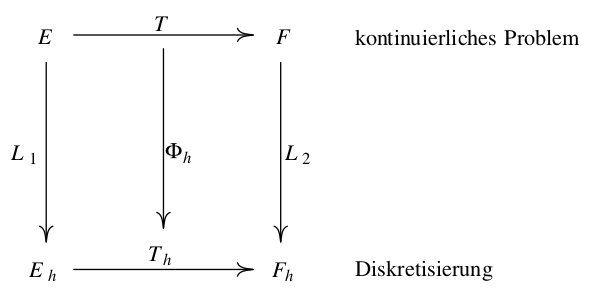
\includegraphics[width=0.45\textwidth]{abstraktkonsistenz.png} \\
	 	Abbildung aus \cite{brokate2016grundwissen} Seite 392
	 \end{figure}
	 Das diskretisierte Problem $ T_h \rho_h = 0  $ heißt genau dann konsistent, wenn für eine analytische Lösung $ \rho^{\star} \in E $ gilt, dass $ \lim\limits_{h \to 0}\lVert \Phi_h(T)L_1\rho^{\star} - L_2T\rho^{\star} \rVert_{F_h} = 0 $.
	 Betrachten wir zunächst in einem Zwischenschritt die Semidiskretisierung (5.3).
	 Die gewählte Herleitung dieser Formulierung soll dabei nahelegen, dass für eine exakte (und glatte) Lösung $ \rho $ die Konsistenz für die Semidiskretisierung erfüllt ist. In oben eingeführter Notation gilt also gerade $ B_h(\rho^{\star},\phi) $ für alle Testfunktionen $ \phi $. Auch wenn es sich bei $ Q_h $ um einen nicht konformen Ansatzraum handelt, ist der Herleitung der Semidiskretisierung dennoch zu entnehmen, dass auch $ B_h(\rho^{\star},\phi_h) $ für alle $ \phi_h \in Q_h $ gilt $(\star)$.  Wichtig ist dabei unter anderem auch die Wahl der numerischen Flussfunktion, der upwind flux erhält aber gerade gewünschten Eigenschaften. 
	 Mehr dazu findet sich in \cite{Har08b}.
	 Für die Zeitdiskretisierung in Form der impliziten Mittelpunktsregel gilt als einstufige Gauß-Quadratur $ \lVert \Phi_h(T)L_1\rho^{\star} - L_2T\rho^{\star} \rVert_{F_h} = O(h^2)$, womit sie insbesondere konsistent ist. \\
	 Daher gilt so für das kombinierte Verfahren, dass eine klassische Lösung $ \rho^{\star} $ somit auch die Volldiskretisierung in obigem Sinne erfüllt. 
\subsubsection{Galerkin Orthogonalität}
Eine direkte Folgerung aus der Konsistenz und $ (\star) $ stellt die Galerkin Orthogonalität dar. Für eine Lösung der Semidiskretisierung $ \rho_h $ und eine analytische Lösung im klassischen Sinne $ \rho^{\star} $ gilt dann nämlich:
\[
 B_h(\rho^{\star}-\rho_h,\phi_h = 0) \quad \forall \phi_h \in Q_h
\]
\subsubsection{Stabilität und Konvergenz}
Die Stabilität ist bei der numerischen Lösung der Transportgleichung einer der wesentlichen Gründe, weswegen wir das Discontinuous Galerkin Verfahren einem Standard-Finite-Elemente-Ansatz vorziehen. Es zeigt sich nämlich, dass ein normales Finite Elemente Verfahren, wie wir es zuvor bei der Lösung des Potentialströmungsproblems genutzt haben, beim Transportproblem instabil ist. Grund dafür ist, dass $ \lVert q \cdot \nabla \rho_h \rVert $ beliebig groß werden kann. Für die DG-Diskretisierung mit upwind flux kann hingegen gezeigt werden, dass die Lösung des Transportproblems stabil ist. Auf eine theoretische Stabilitätsanalyse möchten wir aber an dieser Stelle verzichten und verweisen z.B. auf \cite{Har08b}.
Ebenso wollen wir bezüglich der Konvergenz des Verfahrens auf entsprechende Literatur verweisen. Wir werden später Konvergenzannahmen stellen und diese in entsprechenden Experimenten verifizieren. In der Literatur finden sich aber auch theoretische Konvergenzbeweise, meist unter Verwendung vielfältiger funktionalanalytischer Grundlagen und unter gewissen Regularitätsvoraussetzungen an die bestimmte Lösung. Die theoretische Betrachtung von Discontinuous Galerkinverfahren ist bereits Gegenstand vielfältiger wissenschaftlicher Arbeiten, aber zugleich ein breites Feld, welches noch lange nicht vollständig erforscht ist. \\
%Im nächsten Abschnitt sollen nun schließlich die Überlegungen der letzten Abschnitte gebündelt werden und wir wollen die Multilevel Monte Carlo Methode bei der speziellen Anwendung auf das Transportproblem betrachten.





